\documentclass{article}
\usepackage[utf8]{inputenc}
\usepackage[T1]{fontenc}
\usepackage{csvsimple}
\usepackage{rotating}
\usepackage{graphicx}
\usepackage{amsmath}
\usepackage{listings}
\setlength{\parindent}{0pt}
\title{Symulacje Monte Carlo}
\date{}

\begin{document}

\maketitle
Temat: \textbf{Rozwiązywanie problemu pijanego marynarza}\\
Imię i nazwisko prowadzącego: \textbf{Grzegorz Pawlik}

\begin{center}
\begin{tabular}{|p{5cm}|p{6cm}|}
\hline
$Wykonawca:$ & $Gracjan$ $Tokarz$ $255531$ $W11$  \\
\hline
$Termin$ $zajec:$ & $Piatek , 15:15$\\
\hline
$Data$ $oddania$ $sprawozdania:$ & $23.10.2020r$\\
\hline
\textbf{Ocena	końcowa:} & \\
\hline
\end{tabular}
\end{center}

\textbf{Adnotacje dotyczące wymaganych poprawek,oraz daty otrzymania poprawionego sprawozdania}

\newpage

\section{Kod źródłowy}
\subsection{Drunkard.hpp}
\lstset{
	language=C++
}
\begin{lstlisting}
class Drunkard{

	public:
		Drunkard(long int n, int k);
		~Drunkard(){
			Xn.clear();
		}
		void printToFile();
		double varCalc();

	private:
		long int N, K;
		std::string filepath;
		std::ofstream data;
		std::vector<long int> Xn;
};
\end{lstlisting}

\subsection{Drunkard.cpp}
\begin{lstlisting}
Drunkard::Drunkard(long int n, int k){
	K = k;
	N = n;
	long int x;
	float r;
	filepath = "data.dat";
	std::cout<<K<<" drunks, "<<N<<" steps each\n";
	for (int i = 0; i < K; i++){//iterating drunks
		x = 0;
		for (long int j = 0; j < N; j++){//iterating steps
			r = (float)rand()/RAND_MAX;
			if (r > 0.5) x = x + 1;
			else x = x - 1;
		}
		Xn.push_back(x);
	}
}

void Drunkard::printToFile(){
	data.open(filepath, std::ios_base::app);
	data<<log(N)<<"\t"<<log(varCalc())<<std::endl;
	data.close();
}

double Drunkard::varCalc(){
	long double sqrAvgs = 0;//square of averages
	long double avgSqrs = 0;//average of squares
	for (int i = 0; i < K; i++){
		sqrAvgs += Xn.at(i);
		avgSqrs += Xn.at(i) * Xn.at(i);
	}
	sqrAvgs = sqrAvgs / K;
	sqrAvgs = sqrAvgs * sqrAvgs;
	avgSqrs = avgSqrs / K;
	return avgSqrs - sqrAvgs;
}
\end{lstlisting}

\subsection{main.cpp}
\begin{lstlisting}
int main(int argc, char* argv[], char* envp[]){
	int k = 10000; //number of drunkards
	long int n = atoi(argv[1]); //number of steps
	Drunkard drunkard1(n, k);
	drunkard1.printToFile();
	return 1;
}
\end{lstlisting}

\section{Wyniki}
\begin{center}
\begin{tabular}{l|l}
$\sqrt{N}$ & $\sqrt{\sigma}$\\ \hline
$4.60517$ & $2.29437$\\
$5.29832$ & $2.63724$\\
$5.99146$ & $2.98238$\\
$6.68461$ & $3.32808$\\
$7.37776$ & $3.68327$\\
$8.07091$ & $4.02758$\\
$8.76405$ & $4.38344$\\
$9.4572$ & $4.72663$\\
$10.1503$ & $5.07164$\\
$10.8435$ & $5.41314$\\
$4.60517$ & $2.29437$\\
$5.29832$ & $2.63724$\\
$5.99146$ & $2.98238$\\
$6.68461$ & $3.32808$\\
$7.37776$ & $3.68327$\\
$8.07091$ & $4.02758$\\
$8.76405$ & $4.38344$\\
$9.4572$ & $4.72663$\\
$10.1503$ & $5.07164$\\
$10.8435$ & $5.41314$\\
$11.5366$ & $5.76571$\\
$12.2298$ & $6.12003$\\
$12.9229$ & $6.45345$\\
$13.6161$ & $6.80545$\\
\end{tabular}
\end{center}

\section{Wykresy}
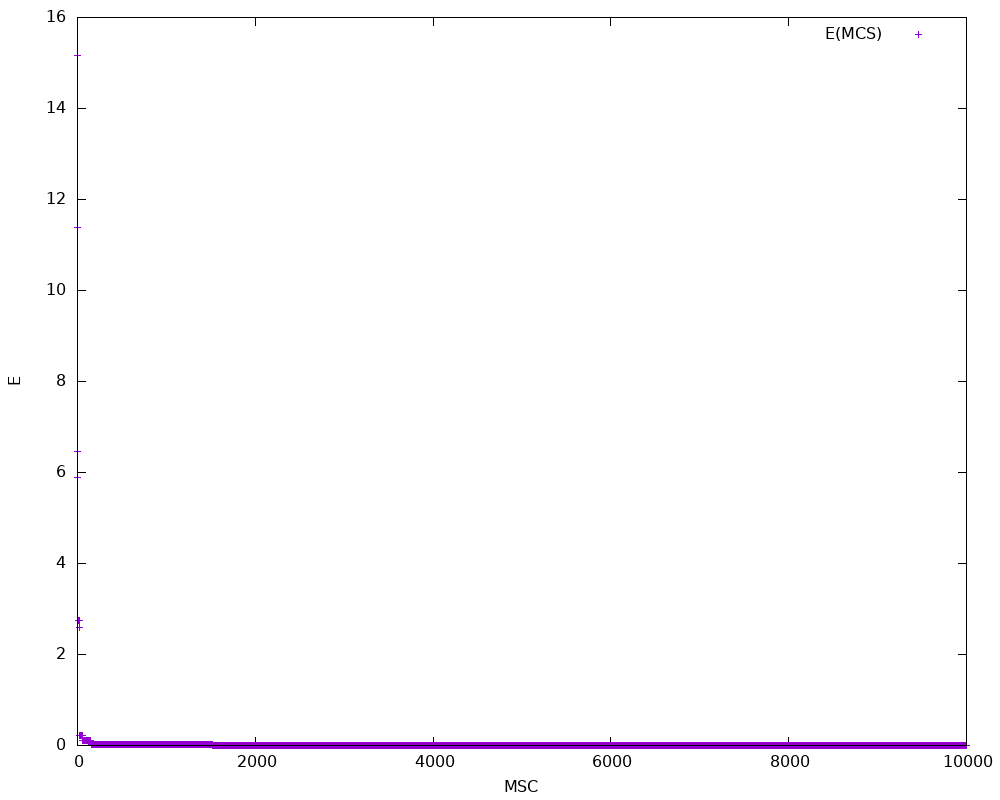
\includegraphics[width=13cm]{plot.png}

\end{document}
